\documentclass[uplatex]{jsarticle}
\usepackage[dvipdfmx]{graphicx}
\usepackage{ascmac}
\usepackage{listings}
\usepackage{amsmath}
\usepackage{bm}
\usepackage{cases}

\DeclareMathOperator*{\minimize}{minimize}


\title{人工知能 課題番号1「人工知能の実現可能性について考察せよ」}
\author{工学部電子情報工学科 03-175001 浅井明里}

\makeatletter
\def\maketitle{%
  \null
  \thispagestyle{empty}%
  \vfill
  \begin{center}\leavevmode
    \normalfont
    {\LARGE \@title\par}%
    \vskip 1cm
    {\Large \@author\par}%
    \vskip 1cm
    {\Large \@date\par}%
  \end{center}%
  \vfill
  \null
  \@thanks%\vfil\null
  \cleardoublepage
  }
\makeatother


\title{人工知能 課題番号17「GAの探索問題」}
\author{工学部電子情報工学科 03-175001 浅井明里}
\date{\today}

\begin{document}
\maketitle

% \section{モンテカルロ探索法とは}
% \subsection{モンテカルロ探索法と従来の手法との相違点}

\section{GAを用いて巡回セールスマン問題の解を探索する}
本課題では、ダーウィン型、ボールドウィン型、ラマルク型の遺伝的アルゴリズム(GA)を用いて巡回セールスマン問題を解き、
得られた解及び探索に要した時間の比較を行なった。

\subsection{巡回セールスマン問題とは}
都市の集合と各2都市間の移動コスト(たとえば距離)が与えられたとき、全ての都市をちょうど一度ずつ巡り出発地に
戻る巡回路の総移動コストが最小のものを求める組合せ最適化問題であり、NP完全である。局所探索アルゴリズムや
焼きなまし法により、一定の解が得られることが示されているが、今回はこの巡回セールスマン問題を遺伝的アルゴリズムにより
探索をする。

\subsection{遺伝的アルゴリズムの概要}
\subsubsection{遺伝的アルゴリズムの流れ}
遺伝的アルゴリズムプログラムの基本的な流れは次のようになる。

\begin{enumerate}
  \item 初期化 \mbox{}\\
  $N$個の個体からなる初期集団を発生させ、各個体の適合度を計算する。通常この初期集団はランダムに生成される。

  \item 各個体の評価 \mbox{}\\\
  各個体の適合度を計算する。この問題で言えば経路全体のコストの大小とし、コストが小さくなるほど
  適合度が高いとする。

  \item 淘汰
  環境に適合しない個体を一定のSelection rateに基づいて淘汰する。仮にSelection rateが0.5であった場合、
  初期化により生成された$N個$の個体のうち、適合率の低い個体は除去される。
  淘汰の方法は以下の二つがある。
  \begin{itemize}
    \item エリート選択 : 単純に,適合度が高い$N$個の個体を残す。局所最適解に陥りやすいので、ルーレット選択と併用する。
    \item ルーレット選択 : 適合度に基づいたルーレット盤を作成し、そのルーレット盤を使用してランダムに選択する方法。
  \end{itemize}
  \item 交叉 \mbox{}\\
  ある親の組み合わせから子を生成する過程。交叉のには様々な手法が存在するが、染色体内に同じ対立遺伝子が現れないようにしたい場合
  (巡回セールスマン問題では同じ都市には複数回訪れない)、部分的交叉法などが活用できる。部分的交叉の実装については実装の項で
  詳述したいと思うが、概要としては、各子供は,各親の遺伝子をそのまま受け継ぐ。
  ランダムに切れ目を選択し切れ目の右側で、同じ位置にある子1と子2の遺伝子を取りだし、
  次に、子1及び子2の染色体上で、この2つの遺伝子の位置を交換する。これを全ての遺伝子に対して実施するというものである。

  \item 突然変異 \mbox{}\\
  ある所与の確率$P_m$でランダムな個体を生成し、集団に追加する。これは局所解から脱出する効果がある。

  \item 生物集団の評価 \mbox{}\\
  収束したか否かの判定を行う。判定方法としては生物集団中の最大の適合度が、ある閾値より
  小さくなった場合や生物集団の適合度の増加率がある閾値以下の世代が一定期間続いた場合、またシンプルに
  世代交代の回数が規定の回数を超えた場合などで判定を行う。収束していない場合には2に戻る。
\end{enumerate}

\subsubsection{ダーウィン型、ボールドウィン型、ラマルク型の遺伝的アルゴリズムの比較}
ダーウィン型、ボールドウィン型、ラマルク型の遺伝的アルゴリズムの特徴はそれぞれ次のようになっている。
\begin{description}
  \item[ダーウィン型]\mbox{}\\
  上述のアルゴリムの流れに従った基本的な遺伝的アルゴリズム。
  \item[ラマルク型]\mbox{}\\
  個体の適合度を評価するため、その個体をスタート地点としてとり、局所解に達するまで山登り法などで局所探索を実施し適合度を
  求める。この局所探索で改良された個体によって子孫が作られることになる。
  \item[ボールドウィン型]\mbox{}\\
  ラマルク型と同様、まず局所解を求めるが、この局所解からそのまま子が作られるのではなく、オリジナルの個体の遺伝子型より子を作成する。
\end{description}
図1はダーウィン型、図2はボールドウィン型、ラマルク型の遺伝的アルゴリズムの流れを図示している。ラマルク型においては直接的に獲得形質が子孫に遺伝することは否定するが、以下の段階を踏むことにより、まるで学習した内容が遺伝子レベルに組み込まれ、
ラマルク効果が発生したように見える。
\begin{enumerate}
  \item 第一段階 : 適応的形質が学習可能なことからメリットを得た個体だ集団中に広まる。
  \item 第二段階 : 学習にかかるコストがより小さい、つまりより生得的に帝王した形質を獲得した個体が集団に広がる。
\end{enumerate}

  \begin{figure}[htbp]
  \begin{minipage}{0.5\hsize}
   \begin{center}
    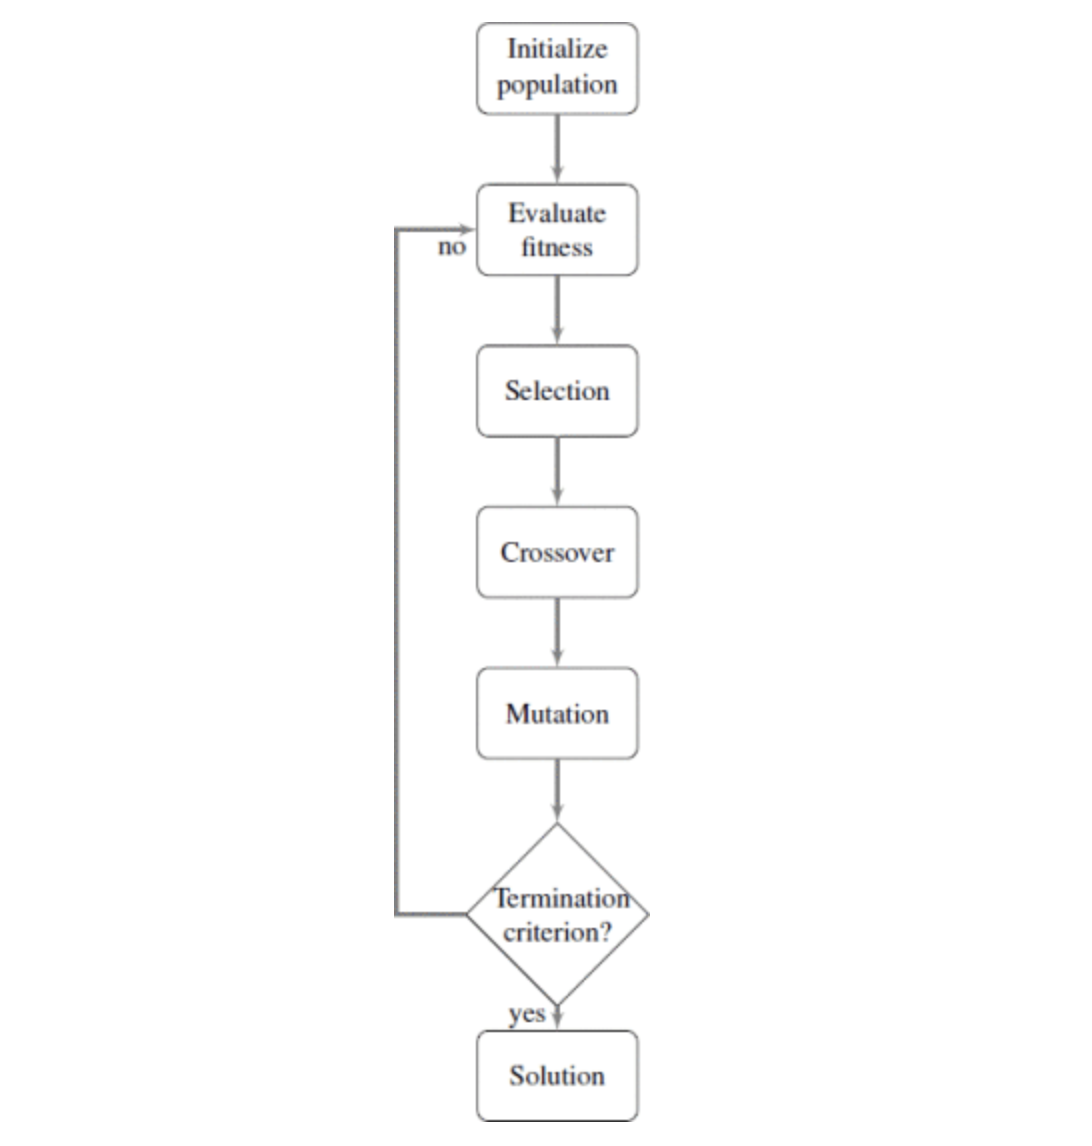
\includegraphics[width=80mm]{darwin.png}
   \end{center}
   \caption{ダーウィン型の遺伝的アルゴリズム}
   \label{fig:one}
  \end{minipage}
  \begin{minipage}{0.5\hsize}
   \begin{center}
    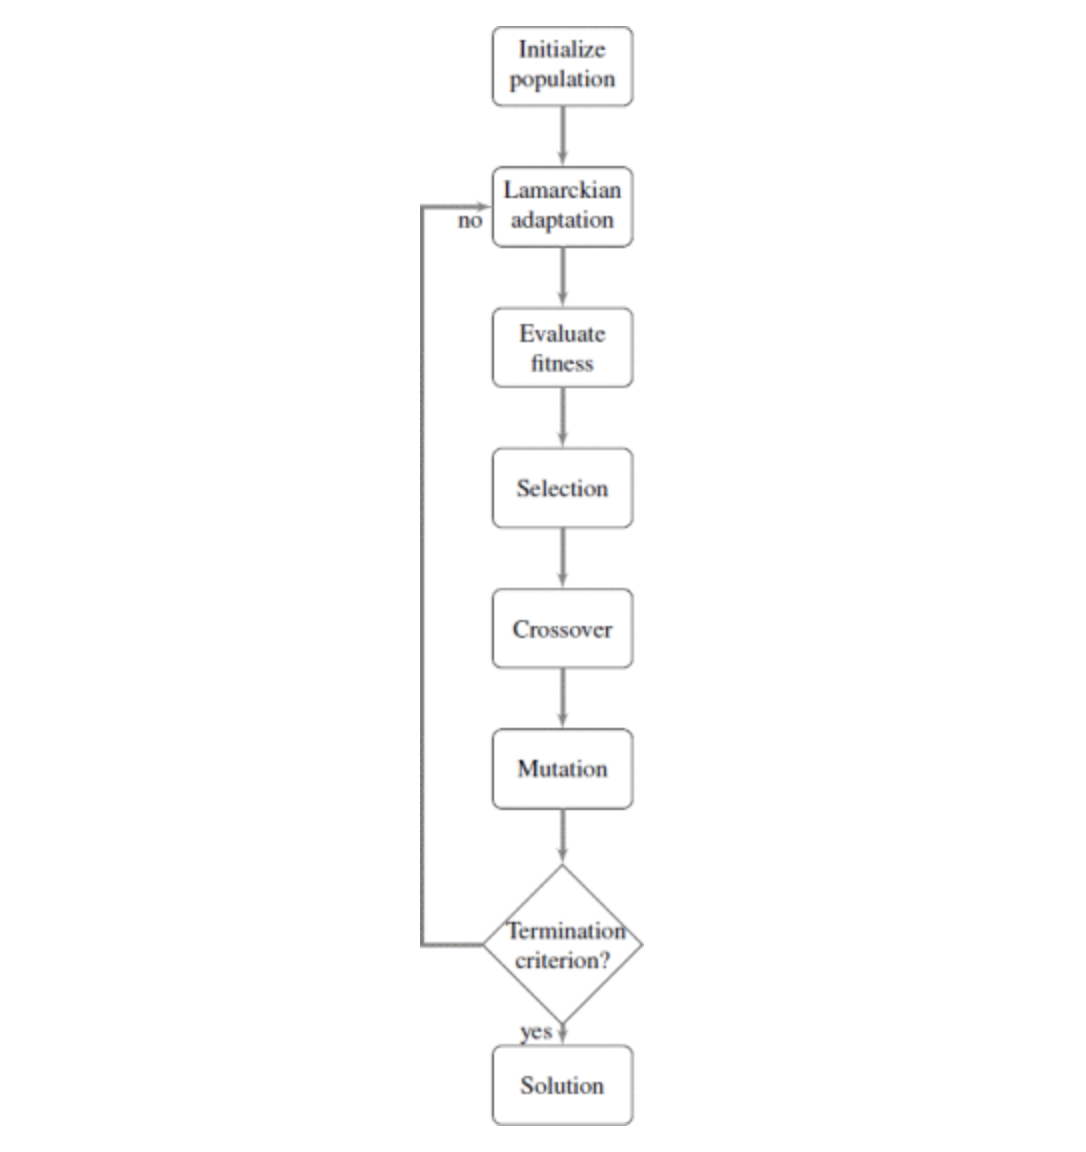
\includegraphics[width=80mm]{baldwin.png}
   \end{center}
   \caption{ボールドウィン型、ラマルク型の遺伝的アルゴリズム}
   \label{fig:two}
  \end{minipage}
  \end{figure}

\section{実装の詳細}
前項の「遺伝的アルゴリズムの流れ」に対応させて実際の実装を説明する。
\subsection{基本の遺伝的アルゴリズムの実装}
\subsubsection{解の初期化}
解の初期化にあたっては、まず$N$個の都市についてつけられたインデックス$i\ (0 \geq i < N)$に従って
巡回する解を一つ生成し、それぞれの世代に含まれる解の最大数、MAX\_POPULATIONの数だけ
これをランダムにシャッフルした初期解を生成する。ここで生成されたMAX\_POPULATION個の初期解は現在の世代を表す
ga\_currentという配列にコピーされる。

\begin{lstlisting}[basicstyle=\ttfamily\footnotesize, frame=single]
void shuffle(int ary[], int size) {
  srand(clock());
  for (int i = 0; i < size; i++) {
    int j = rand() % size;
    int t = ary[i];
    ary[i] = ary[j];
    ary[j] = t;
  }
}

void create_initial_generation(int n) {
  int *temp = malloc(n * sizeof(int));
  for (int i = 0; i < MAX_POPULATION; i++) {
    size_t size = n * sizeof(int);
    memcpy(temp, result, size);
    shuffle(temp, n);
    // 生成されたランダムな個体を現世代の配列にコピーする。
    copy_population_to_generation(temp, i, n);
  }
}
\end{lstlisting}

\subsubsection{各個体の評価}
次に得られた解に対して、その適合度を評価する。巡回セールスマン問題においては全ての都市を回る
最小コストの経路を探索することが目的であるため、ここでは適合度として
それぞれの経路の総距離を計算し、適合度とする。次にこの適合度の小さい方から昇順になるように
現世代の個体(全ての都市を回るための経路)を並び替える。

\begin{lstlisting}[basicstyle=\ttfamily\footnotesize, frame=single]
  void sort_population_by_fitness(int n, double fitness[MAX_POPULATION]) {
    int i, j;

    for (i = 0; i < MAX_POPULATION; i++) {
      for (j = MAX_POPULATION - 1; j > i; j--) {
        if (fitness[j] < fitness[j - 1]) {
          ...
          // Sort ga_corrent by fitness score.
          size_t size = n * sizeof(int);
          int *tmp = malloc(size);
          memcpy(tmp, ga_current[j], size);

          for (int k = 0; k < n; k++) {
            ga_current[j][k] = ga_current[j - 1][k];
          }
          for (int k = 0; k < n; k++) {
            ga_current[j - 1][k] = tmp[k];
          }
          free(tmp);
        }
      }
    }
  }

  void evalution(int n) {
    double fitness[MAX_POPULATION];
    for (int i = 0; i < MAX_POPULATION; i++) {
      fitness[i] = calculate_distance(ga_current[i], n);
    }
    sort_population_by_fitness(n, fitness);
  }
\end{lstlisting}

\subsubsection{選択、交叉、突然変異}
次に、選択、交叉、突然変異を行い、次世代の個体を生成する。

まず、適合度の高い個体については、
そのまま次世代に引き継がれる。プログラムでは、適合度でソートした時にその順位が
MAX\_POPULATION * elite\_rate以下になるものについてはこの選択を適用した。

次に、一定割合でランダムな突然変異を発生させて局所解にスタックしないよう、ある一定割合で
初期個体の生成時に行ったのと同様の手法によりランダムな解を生成した。

最後に、現世代から$M$個の親のペアを作成し、一つのペアから2個、すなわち合計$2M$個の個体を交叉によって生成し、
次世代に追加する。

\begin{lstlisting}[basicstyle=\ttfamily\footnotesize, frame=single]
void generate_new(int n) {
  for (int i = 0; i < MAX_POPULATION; i = i + 2) {
    if (i < elite_rate * MAX_POPULATION) {
      // Selection
      copy_parent_to_child(i, i, n);
      copy_parent_to_child(i + 1, i + 1, n);
    } else if (i < (elite_rate + mutation_rate) * MAX_POPULATION) {
      // Mutation
      int *tmp = malloc(n * sizeof(int));
      size_t size = n * sizeof(int);
      memcpy(tmp, result, size);
      for (int j = 0; j < n; j++) {
        int k = rand() % n;
        int t = tmp[j];
        ga_next[i][j] = tmp[k];
        temp[k] = t;
      }
      ...
    } else {
      //Cross Over
      int parent1_id = rand() % MAX_POPULATION;
      int parent2_id = rand() % MAX_POPULATION;
      if (parent2_id == parent1_id) {
        if (parent1_id == 0) {
          parent2_id = rand() % MAX_POPULATION;
        } else {
          parent2_id = rand() % parent1_id;
        }
      }
      crossover(parent1_id, parent2_id, i, i + 1, n);
    }
  }
}
\end{lstlisting}

交叉においては、前述の通り部分交叉法を用いている。部分交叉は以下のステップで実行される。
\begin{enumerate}
  \item 前半と後半の境界をランダムに決定する。(下記プログラムにおけるswitch\_digit)
  \item まず、現世代の前半部分については、それぞれ対応する次世代の前半部分にそのままコピーする。
  \item また現世代の個体の後半部分については、一旦別の配列に格納する。(下記プログラムにおけるparent1\_rest及び
  parent2\_rest)
  \item 次世代の新しい個体それぞれの後半部分は、2でコピーした親と異なる親のある数字から自身のコピーした親の後半部分と
  一致するものを順に見つけ、元の親の後半部分の$j$番目で発見した際には、もう一方の後半配列の同じく$j$番目をこの
  次世代の個体の配列に追加する。
  \item これを配列長が都市の長さ$N$となるまで繰り返す。
\end{enumerate}

\begin{lstlisting}[basicstyle=\ttfamily\footnotesize, frame=single]
void crossover(int parent1_index, int parent2_index, int child1_index,
               int child2_index, int n) {
  int switch_digit = rand() % n;

  int *parent1_rest = malloc(n * sizeof(int));
  int *parent2_rest = malloc(n * sizeof(int));

  for (int i = 0; i < n; i++) {
    if (i < switch_digit) {
      ga_next[child1_index][i] = ga_current[parent1_index][i];
      ga_next[child2_index][i] = ga_current[parent2_index][i];
    } else {
      parent1_rest[i - switch_digit] = ga_current[parent1_index][i];
      parent2_rest[i - switch_digit] = ga_current[parent2_index][i];
    }
  }

  int child1_digit = switch_digit;
  int child2_digit = switch_digit;

  for (int i = 0; i < n; i++) {
    for (int j = 0; j < n - switch_digit; j++) {
      if (ga_current[parent2_index][i] == parent1_rest[j]) {
        ga_next[child1_index][child1_digit] = parent2_rest[j];
        child1_digit++;
      }

      if (ga_current[parent1_index][i] == parent2_rest[j]) {
        ga_next[child2_index][child2_digit] = parent1_rest[j];
        child2_digit++;
      }
    }
  }
}
\end{lstlisting}


\subsubsection{生物集団の評価}
今回は収束したか否かの判定条件について、世代交代が5万回となるまで終了しないとした。

\subsection{ラマルク型、ボールドウィン型における獲得形質の学習について}
ラマルク型、ボールドウィン型では共に「まず局所解を求め、それを何らかの形で次世代に継承する」ことを行う。
今回は、ダーウィン型のようにランダムで生成された初期解をまず山登り法により改善し、
ラマルク型では全ての個体に対してこの改善を行い、この改善された個体から上述の方法により次世代を生成した。
またボールドウィン型については現世代の個体に対して一定割合で局所解を求めて解を改善し、
残りについてはそのままとした上で、次世代を生成した。これにより、全ての個体がある獲得形質を
直接継承しているわけではないが、ある程度学習された個体の集団全体に占める割合が徐々に高まることにより、
ある獲得形質がまるで遺伝的に継承されているようなボールドウィン効果を得ることができる。

\begin{lstlisting}[basicstyle=\ttfamily\footnotesize, frame=single]
void improve_route_ver2(int n, int ga_idx) {
  // 山登り法により、解を改善する。
  srand((unsigned)time(NULL));
  int count = 0;
  int temp[MAX_CITIES];
  double distance1;
  double distance2;
  while (count < 100) {
    int c0 = random_integer(n);
    int c1 = random_integer(n);
    if (c0 != c1) {
      distance1 = calculate_distance(ga_current[ga_idx], n);
      swap(&ga_current[ga_idx][c0], &ga_current[ga_idx][c1]);
      distance2 = calculate_distance(ga_current[ga_idx], n);
      if (distance2 > distance1) {
        swap(&ga_current[ga_idx][c0], &ga_current[ga_idx][c1]);
      }
      count++;
    }
  }
}
// 次世代の生成を行う前にまずそれぞれの局所解を求める。
void lamarkian_adaptation(int n, int is_baldwin){
  int num_improve = is_baldwin? MAX_POPULATION * baldwin_rate : MAX_POPULATION;
  for (int i = 0; i < num_improve; i++){
    improve_route_ver2(n, i);
  }
}
\end{lstlisting}


\subsection{プログラムの実行}
ダーウィン型の遺伝的アルゴリズムプログラムはtsp\_darwin.cppに、ボールドウィン、ラマルク型についてはtsp\_lamrk\_baldwin.cに実装されている。
以下のコマンドを入力すると、全ての都市を1からN番目まで順に巡回した場合の初期解のコストとGAで求められた解のコストを確認することができる。
第1引数で都市の数を指定する。

\begin{lstlisting}[basicstyle=\ttfamily\footnotesize, frame=single]
  $ gcc tsp_darwin.cpp
  $ ./a.out 10
\end{lstlisting}

ラマルク型の遺伝的アルゴリズムの実行のためには以下のコマンドを入力する。この時、第2引数は実行するプログラムがラマルク型か
ボールドウィン型か確認するフラッグである。

\begin{lstlisting}[basicstyle=\ttfamily\footnotesize, frame=single]
  $ gcc tsp\_lamrk\_baldwin.c
  $ ./a.out 10 0
\end{lstlisting}
\begin{lstlisting}[basicstyle=\ttfamily\footnotesize, frame=single]
  $ ./a.out 10 1
\end{lstlisting}
また別ターミナルで実行前に以下のコマンドを入力すると、実行の結果得られたルートを可視化できる。
この可視化の部分については昨年のソフトウェア2課題の巡回セールスマン問題課題より引用した。
なお、ソフトウェア2課題においては焼きなまし法やNearest Neighborなどの実装を行なったため、
遺伝的アルゴリズムに関連する全てのプログラムについては今回課題で初めて実装をした。

\begin{lstlisting}[basicstyle=\ttfamily\footnotesize, frame=single]
  $ tail -f map.txt
\end{lstlisting}

\section{結果の比較}
以上のプログラムを年の数を$N = 6,\ 8,\ 10,\ 12,\ 14,\ 16,\ 18,\ 22$と変化させた上でコスト及び実行時間が
どう変化するかを観測した。コストの年の数に対する推移については次の図3で示している。このグラフからもわかるように、
学習収束条件を「ある一定回以上世代交代を繰り返した」としていたために、特にダーウィン型では
年の増加に伴い想定される解の数が爆発的に増加する中でよりコストの少ない解を見つけにくくなっている様子が観測できる。
一方ラマルク、ボールドウィン型では解がせいぜい20個程度では全ての個体が局所解、もしくは一定割合が局所解となった個体の集団
から次世代を生成していくことにより、効率的に「学習」し、よりコストの少ない経路を求められていることがわかる。
前述のように判定条件を決めうちしているため、アルゴリズムごとの都市数の増加による計算時間の変動はあまり大きくはないが、
ダーウィン型と比較し次世代を生成する以前に毎回局所問題を解く必要のあるラマルク型、ボールドウィン型はやはり実行時間は長くなる。

\begin{figure}
  \begin{center}
    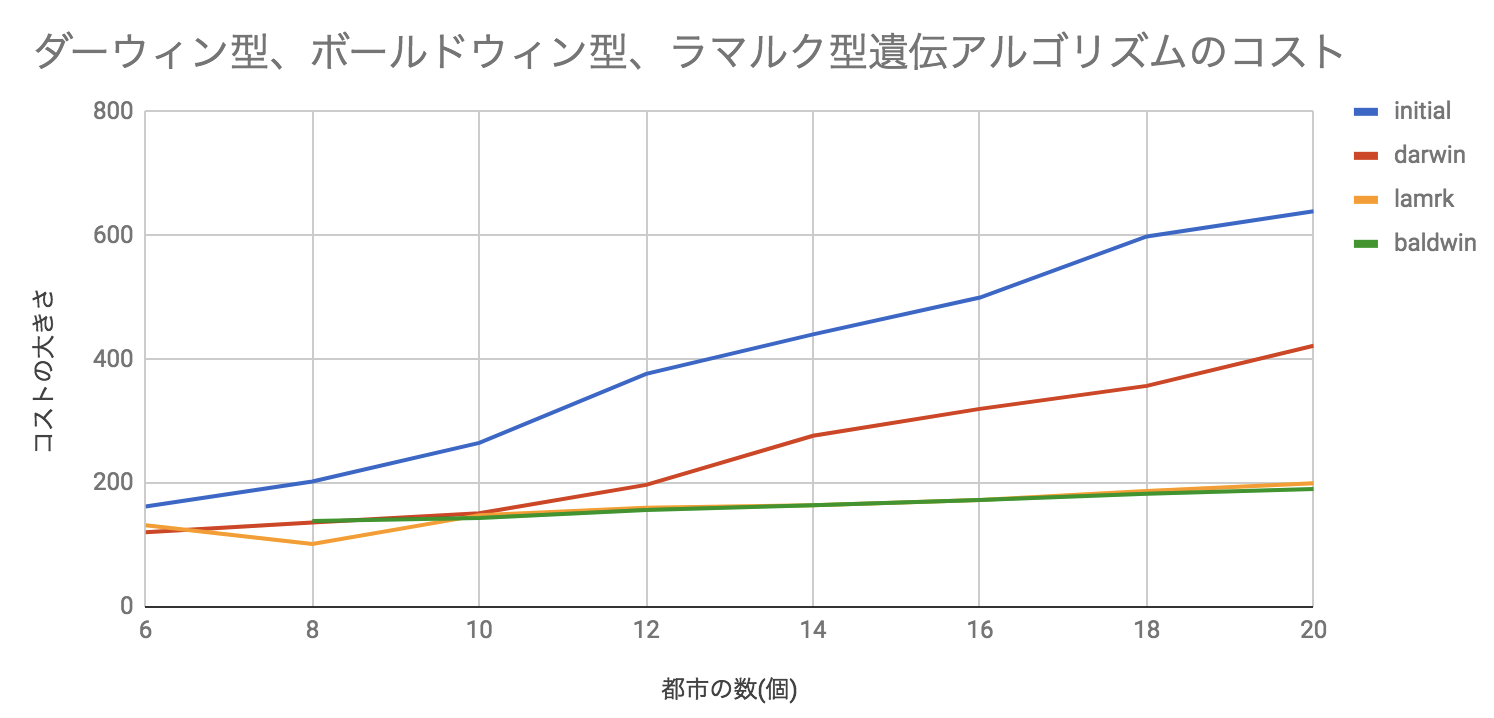
\includegraphics[width=17cm]{ga_cost.png}
    \caption{遺伝的アルゴリズムのコストの比較}
  \end{center}
\end{figure}

\begin{thebibliography}{9}
  \bibitem{evans} Andreas Holzinger, David Blanchard, Vasile Palade, Raul Rabadan.
    "Darwin, Lamarck, or Baldwin: Applying Evolutionary Algorithms to Machine Learning Techniques",  IEEE/WIC/ACM International Joint Conferences on Web Intelligence (WI) and Intelligent Agent Technologies (IAT), 2014.
  \bibitem{iba} 伊庭斉志,
    『進化計算と深層学習 -創発する知能』, オーム社 , 2015.
  \bibitem{suganuma}菅沼義昇「システムの最適化 -4. 遺伝的アルゴリズム(GA : Genetic Algorithm)- 」, https://www.sist.ac.jp/~suganuma/kougi/other\_lecture/SE/opt/GA/GA.htm
\end{thebibliography}


\end{document}
